\chapter{Desenvolvimento}
\label{cap:desenvolvimento}

Este capítulo apresenta a implementação prática dos componentes definidos na metodologia, detalhando o desenvolvimento da API de controle Fuzzy, da Interface Humano-Máquina (IHM) e da integração via protocolo OPC UA. O desenvolvimento seguiu uma abordagem modular, onde cada componente foi implementado e testado individualmente antes da integração final, garantindo funcionalidade e robustez do sistema completo.

A implementação baseia-se na arquitetura distribuída proposta, onde a API de controle Fuzzy desenvolvida em Python atua como núcleo inteligente, a IHM em C\# proporciona interface de supervisão e controle, e a comunicação OPC UA garante interoperabilidade e padronização na troca de dados. Esta estrutura modular facilita manutenção, permite expansões futuras e assegura conformidade com padrões industriais estabelecidos.

\section{Protocolo de comunicação OPC}
\label{sec:opc}

O protocolo OPC UA (OPC Unified Architecture) constitui a base fundamental de comunicação da arquitetura proposta, proporcionando interoperabilidade e padronização na troca de dados entre a planta de nível simulada e a IHM. O OPC (Open Platform Communications) representa um conjunto de especificações padronizadas que definem a interface entre clientes e servidores em sistemas de automação industrial, facilitando a comunicação entre dispositivos de hardware e software de diferentes fornecedores \cite{opc2025a}.

O desenvolvimento do OPC UA surge como evolução natural do OPC Classic, criado para superar limitações fundamentais dos protocolos proprietários que resultavam em "ilhas de automação" isoladas. O OPC UA fundamenta-se em uma arquitetura orientada a serviços que separa claramente a funcionalidade de aplicação dos detalhes específicos da tecnologia de comunicação subjacente, proporcionando flexibilidade excepcional e operação independente de plataforma, sistema operacional ou tecnologia de rede utilizada \cite{opc2025b}.

A arquitetura OPC UA estrutura-se em múltiplas camadas funcionais que garantem robustez e versatilidade na comunicação industrial. A \textbf{camada de transporte} suporta múltiplos protocolos de comunicação incluindo TCP/IP binário nativo, HTTPS e WebSockets, permitindo implementação desde dispositivos embarcados até aplicações em nuvem. A \textbf{camada de serialização} oferece codificação binária otimizada para eficiência máxima e codificação JSON/XML para facilitar integração web e interoperabilidade ampliada \cite{opc2025b}.

O \textbf{modelo de informação orientado a objetos} constitui o núcleo conceitual inovador do OPC UA, definindo estruturação hierárquica de dados através de espaço de endereçamento baseado em nós interconectados por referências tipificadas. Este modelo permite representação rica e semântica de informações industriais, suportando desde variáveis simples até modelos complexos de equipamentos e processos. Os tipos fundamentais incluem \textbf{Object Nodes} para entidades físicas ou lógicas, \textbf{Variable Nodes} para dados de processo, \textbf{Method Nodes} para operações remotas e \textbf{DataType Nodes} para definições estruturadas \cite{opc2025b}.

O protocolo implementa paradigma cliente-servidor robusto onde servidores OPC UA expõem funcionalidades através de espaços de endereçamento estruturados, enquanto clientes acessam informações mediante serviços padronizados. O processo de estabelecimento de conexão segue rigorosamente especificações IEC 62541, iniciando com \textbf{descoberta automática de endpoints}, seguida por \textbf{estabelecimento de canal seguro} com negociação de políticas de segurança e \textbf{criação de sessão autenticada} com controle de acesso baseado em certificados.

A estratégia de comunicação baseia-se em \textbf{mecanismo de assinatura (subscription)} que permite monitoramento eficiente em tempo real. Servidores notificam automaticamente clientes sobre modificações de valores, eliminando polling desnecessário e otimizando utilização de largura de banda. O sistema suporta configuração granular de taxas de amostragem, filtros de dados e políticas de entrega, permitindo otimização específica para cada aplicação industrial.

A característica distintiva do OPC UA reside na \textbf{interoperabilidade universal} que opera independentemente de plataforma, sistema operacional ou fornecedor. Esta independência tecnológica elimina vendor lock-in e facilita integração de sistemas heterogêneos, aspecto fundamental para implementação da Indústria 4.0. A padronização rigorosa pela OPC Foundation assegura compatibilidade entre implementações diversas, promovendo ecossistema industrial aberto e competitivo que suporta desde dispositivos embarcados até aplicações empresariais em nuvem \cite{opc2025b}.

\section{Modificação da Planta para utilização do OPC}
\label{sec:opcmodificado}

A integração da planta de nível do Matlab/Simulink com o protocolo OPC UA requer modificações estruturais específicas para possibilitar a comunicação padronizada com sistemas externos. O modelo original \textbf{sltank} foi concebido como sistema de simulação fechado, sendo necessária sua adaptação para exposição de variáveis de processo através de interface OPC UA, garantindo interoperabilidade com a arquitetura distribuída proposta.

A necessidade de modificação surge das limitações inerentes ao modelo original, que não possui capacidades nativas de comunicação externa além do ambiente Simulink. A arquitetura distribuída requer exposição controlada de variáveis críticas do processo através de servidor OPC UA, permitindo que clientes externos possam monitorar variáveis de processo em tempo real e enviar comandos de controle para atuação na planta simulada.

As modificações implementadas concentram-se na adição de blocos especializados para comunicação OPC, mantendo integridade do modelo matemático original. O \textbf{OPC Configuration Block} constitui o componente principal da modificação, garantindo a configuração e conexão com o servidor OPC UA. Adicionalmente, foram incorporados blocos específicos para operações de leitura e escrita de dados via protocolo OPC UA.

O \textbf{bloco OPC Read} permite a seleção sistemática de tags para leitura de dados provenientes do servidor OPC. As tags selecionadas para operação de leitura incluem \textbf{Output} (saída do valor calculado pela API de controle Fuzzy) e \textbf{Setpoint} (nível de referência para controle). Esta configuração possibilita que a planta receba comandos de controle calculados externamente pela API Fuzzy e valores de referência definidos pelo operador através da IHM.

\begin{figure}[H]
    \centering
    \caption[Configuração do bloco OPC Read para leitura de tags do servidor OPC.]{Configuração do bloco OPC Read para leitura de tags do servidor OPC.}
    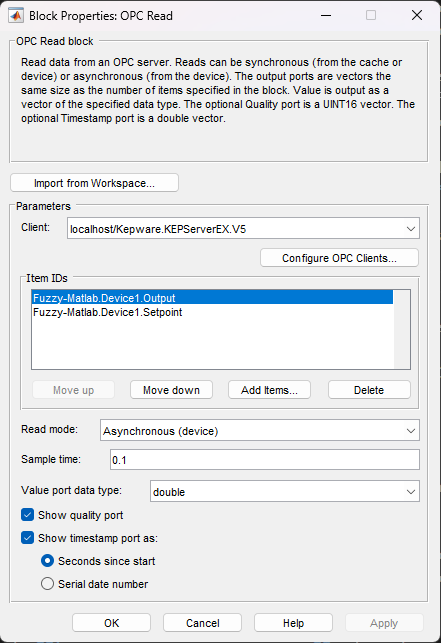
\includegraphics[width=0.5\textwidth]{figuras/imagens/opc-read.png}
    
    {Fonte: Dias, 2025.}
    \label{fig:opcread}
\end{figure}

O \textbf{bloco OPC Write} implementa funcionalidade complementar, permitindo a seleção de tags para escrita de dados da planta para o servidor OPC. As tags configuradas para operação de escrita compreendem \textbf{Error} (erro medido entre setpoint e nível atual), \textbf{Rate} (variação temporal do erro) e \textbf{Level} (nível atual de água no tanque). Esta configuração garante que o cliente OPC UA tenha acesso contínuo às variáveis de processo necessárias para cálculo do controle Fuzzy.

\begin{figure}[H]
    \centering
    \caption[Configuração do bloco OPC Write para escrita de tags no servidor OPC.]{Configuração do bloco OPC Write para escrita de tags no servidor OPC.}
    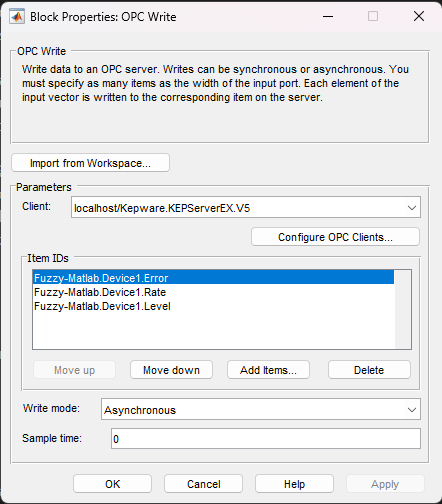
\includegraphics[width=0.5\textwidth]{figuras/imagens/opc-write.png}
    
    {Fonte: Dias, 2025.}
    \label{fig:opcwrite}
\end{figure}

A configuração bidirecional dos blocos OPC Read e OPC Write estabelece ciclo fechado de comunicação entre a planta simulada e o sistema de controle externo. O fluxo de dados iniciado pela escrita das variáveis de processo (Error, Rate, Level) pelo bloco OPC Write é consumido pela API de controle Fuzzy através da IHM, que processa estas informações e retorna comando de controle (Output) juntamente com valor de setpoint atualizado, dados estes lidos pelo bloco OPC Read para atuação na planta.

A estrutura hierárquica do espaço de endereçamento OPC UA implementada segue convenções industriais padrão, organizando as variáveis de processo em namespace específico com identificadores únicos descritivos. A Tabela 1 apresenta o mapeamento completo entre as variáveis de processo e suas respectivas tags OPC UA no servidor.

\begin{table}[H]
\centering
\caption{Mapeamento de variáveis de processo para tags OPC UA}
\begin{adjustbox}{max width=\textwidth}
\begin{tabular}{|l|l|l|l|}
\hline
\textbf{Variável de Processo} & \textbf{Tipo} & \textbf{Tag OPC UA} & \textbf{Descrição} \\
\hline
Error     & Write & Fuzzy-Matlab.Device1.Error     & Erro medido entre setpoint e nível atual \\
Rate      & Write & Fuzzy-Matlab.Device1.Rate      & Variação temporal do erro \\
Level     & Write & Fuzzy-Matlab.Device1.Level     & Nível atual de água no tanque \\
Output    & Read  & Fuzzy-Matlab.Device1.Output    & Saída do valor calculado pela API Fuzzy \\
Setpoint  & Read  & Fuzzy-Matlab.Device1.Setpoint  & Nível de referência para controle \\
\hline
\end{tabular}
\end{adjustbox}
\label{tab:tags-opc-ua}
\end{table}

A nomenclatura adotada utiliza o prefixo \textbf{Fuzzy-Matlab.Device1} seguido pelo identificador específico da variável, proporcionando organização lógica e facilitando identificação das tags pelos clientes OPC UA. Esta estrutura permite expansão futura do sistema através da adição de novos dispositivos (Device2, Device3, etc.) sem conflitos de nomenclatura.

A implementação completa dessas modificações resulta na configuração final da planta mostrada na figura abaixo, onde é possível visualizar a integração dos blocos OPC no modelo original, mantendo a funcionalidade matemática do sistema enquanto adiciona capacidades de comunicação externa padronizada.

\begin{figure}[H]
    \centering
    \caption[Planta de nível modificada com integração OPC UA para comunicação externa.]{Planta de nível modificada com integração OPC UA para comunicação externa.}
    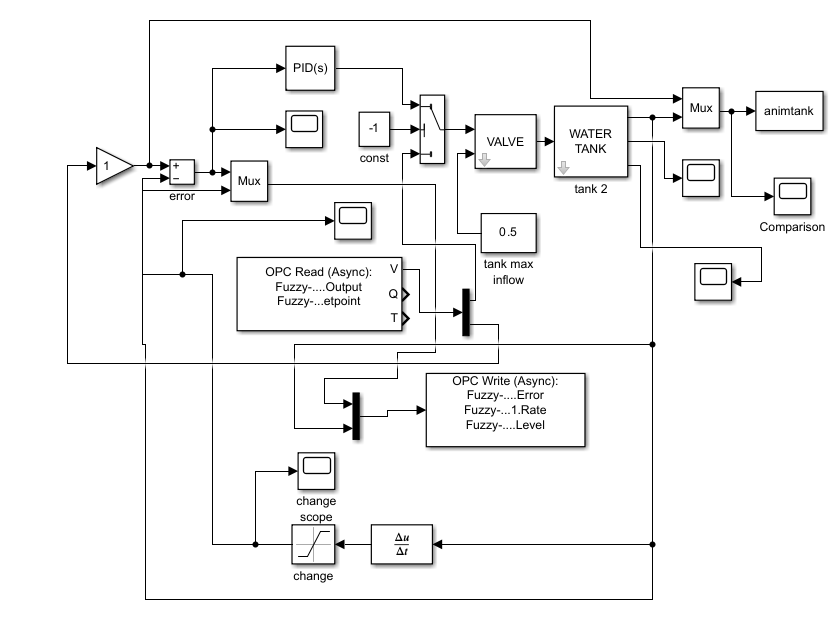
\includegraphics[width=1\textwidth]{figuras/imagens/planta-opc.png}
    
    {Fonte: Dias, 2025.}
    \label{fig:plantaopc}
\end{figure}

\section{Controlador Fuzzy}
\label{sec:controfuzzy}

A lógica Fuzzy representa uma extensão da lógica booleana clássica, permitindo o tratamento de informações imprecisas e incertas através de conjuntos difusos que possibilitam transições graduais entre estados lógicos. Diferentemente da lógica convencional que opera exclusivamente com valores binários (0 ou 1), a lógica Fuzzy admite graus de pertinência intermediários no intervalo [0,1], proporcionando modelagem mais próxima do raciocínio humano e adequada para sistemas complexos com comportamento não linear \cite{zadeh1965}.

O controle Fuzzy fundamenta-se na capacidade de incorporar conhecimento heurístico especializado diretamente no algoritmo de controle, dispensando a necessidade de modelos matemáticos rigorosos do processo. Esta característica torna-se particularmente vantajosa em sistemas de controle de nível, onde não linearidades, tempo morto e variações paramétricas dificultam a aplicação eficaz de técnicas de controle convencionais. A abordagem Fuzzy permite que operadores experientes codifiquem seu conhecimento empírico em regras linguísticas intuitivas, resultando em controladores robustos e de fácil ajuste \cite{mamdani1975}.

A necessidade de implementar o controlador Fuzzy em ambiente Python surge da arquitetura distribuída proposta, onde a lógica de controle opera como serviço independente acessível via API REST. O modelo original \textbf{sltank} do Matlab implementa controle Fuzzy nativo através da ferramenta Fuzzy Logic Designer, sendo necessária a extração e adaptação desses parâmetros para implementação em Python utilizando bibliotecas especializadas como \textbf{scikit-fuzzy}. Esta migração preserva a funcionalidade de controle original enquanto proporciona flexibilidade arquitetural e independência tecnológica \cite{mathWorks2025}.

O controlador Fuzzy implementado utiliza arquitetura de inferência Mamdani com duas variáveis de entrada e uma variável de saída, seguindo a parametrização extraída do exemplo de referência. As \textbf{variáveis de entrada} compreendem o erro de nível (diferença entre setpoint e nível atual) e a taxa de variação do erro (derivada temporal do erro), enquanto a \textbf{variável de saída} corresponde ao sinal de controle da válvula de entrada.

A definição das funções de pertinência segue critérios específicos baseados nas características do processo e na natureza das variáveis envolvidas. As \textbf{variáveis de entrada} (level e rate) utilizam \textbf{funções de pertinência gaussianas}, que proporcionam transições suaves entre os conjuntos difusos e melhor representação da incerteza inerente às medições de processo. As funções gaussianas são caracterizadas pela sua forma em sino, definidas pelos parâmetros de centro e largura, oferecendo gradações naturais que refletem fielmente a imprecisão típica de sensores industriais.

A \textbf{variável de saída} (valve) emprega \textbf{funções de pertinência triangulares}, apropriadas para representar ações de controle discretas e bem definidas. Esta escolha justifica-se pela necessidade de comandos de controle precisos para a válvula, onde a forma triangular proporciona delimitação clara entre diferentes intensidades de atuação, facilitando a interpretação e implementação das ações de controle.

\begin{figure}[H]
    \centering
    \caption[Funções de pertinência gaussianas da variável de entrada "level" (erro de nível).]{Funções de pertinência gaussianas da variável de entrada "level" (erro de nível).}
    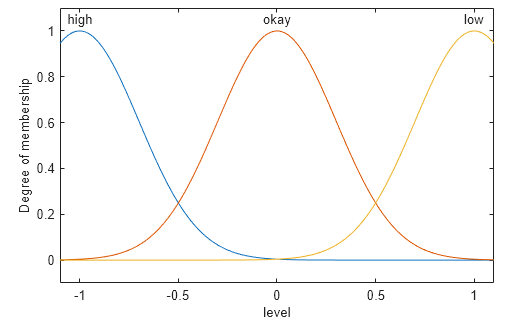
\includegraphics[width=1\textwidth]{figuras/imagens/level.png}
    
    {Fonte: Dias, 2025.}
    \label{fig:fuzzylevel}
\end{figure}

\begin{figure}[H]
    \centering
    \caption[Funções de pertinência gaussianas da variável de entrada "rate" (taxa de variação).]{Funções de pertinência gaussianas da variável de entrada "rate" (taxa de variação).}
    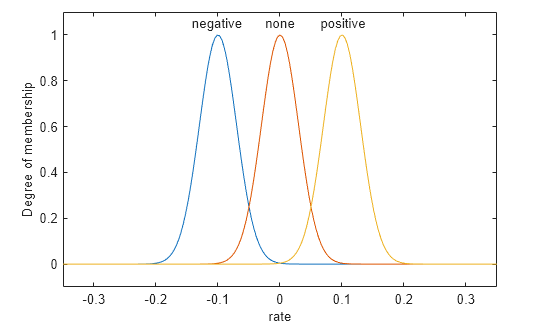
\includegraphics[width=1\textwidth]{figuras/imagens/rate.png}
    
    {Fonte: Dias, 2025.}
    \label{fig:fuzzyrate}
\end{figure}

\begin{figure}[H]
    \centering
    \caption[Funções de pertinência triangulares da variável de saída "valve" (sinal de controle).]{Funções de pertinência triangulares da variável de saída "valve" (sinal de controle).}
    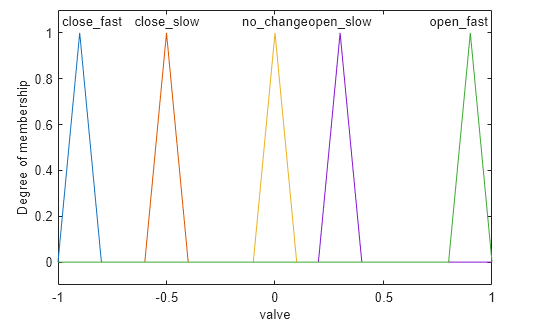
\includegraphics[width=1\textwidth]{figuras/imagens/valve.png}
    
    {Fonte: Dias, 2025.}
    \label{fig:fuzzyvalve}
\end{figure}

O sistema de regras Fuzzy implementado baseia-se em conhecimento heurístico especializado sobre controle de nível, contemplando cinco regras fundamentais que capturam a essência do comportamento desejado do controlador:

\begin{itemize}
\item Regra 1: Se o nível está Ok, então a válvula não é ajustada (\( \sigma \): 0,3; \( \mu \): 0)
Esta regra estabelece a condição de equilíbrio, onde pequenos desvios em torno do setpoint não resultam em ações de controle significativas, evitando oscilações desnecessárias e garantindo estabilidade em regime permanente. Os parâmetros da função gaussiana definem um desvio padrão de 0,3 centrado em zero.
\item Regra 2: Se o nível está Low, então abra a válvula rapidamente (\( \sigma \): 0,3; \( \mu \): 1)
Implementa ação corretiva intensa para situações de nível baixo, aumentando significativamente a vazão de entrada para recuperação rápida do nível desejado, priorizando a segurança operacional e evitando operação em vazio. A função gaussiana apresenta desvio padrão de 0,3 centrada em 1.
\item Regra 3: Se o nível está High, então feche-a rapidamente (\( \sigma \): 0,3; \( \mu \): -1)
Estabelece resposta imediata para condições de nível elevado, reduzindo drasticamente a vazão de entrada para prevenir transbordamentos e manter o processo dentro dos limites operacionais seguros. A parametrização gaussiana utiliza desvio padrão de 0,3 centrado em -1.
\item Regra 4: Se o nível está Ok e aumentando, então feche a válvula devagar
Incorpora comportamento antecipativo baseado na taxa de variação, aplicando correção preventiva quando o nível aproxima-se do setpoint com tendência ascendente, evitando ultrapassagem excessiva.
\item Regra 5: Se o nível está Ok e decrescendo, então abra a válvula devagar
Complementa o comportamento antecipativo para tendência descendente, proporcionando correção suave quando o nível está próximo do setpoint mas apresenta tendência de redução.
\end{itemize}

onde, 

\begin{itemize}
    \item \( \sigma \) é o desvio padrão (sigma) das funções de pertinência gaussianas.
    \item \( \mu \) é o valor médio (mu) das funções de pertinência gaussianas.
\end{itemize}

Esta estrutura de regras implementa estratégia de controle híbrida que combina \textbf{ação corretiva proporcional} ao erro medido com \textbf{comportamento antecipativo} baseado na derivada temporal, resultando em controlador robusto capaz de lidar eficazmente com as características não lineares do processo de controle de nível.

\section{API de controle Fuzzy}
\label{sec:apicontrolefuzzy}

A implementação da API de controle Fuzzy constitui o núcleo computacional inteligente da arquitetura distribuída proposta, responsável por materializar os conceitos teóricos de lógica Fuzzy em uma aplicação prática acessível via protocolo HTTP/REST. Esta API representa a tradução dos parâmetros e regras definidos anteriormente em código Python executável, proporcionando interface padronizada para integração com sistemas industriais heterogêneos.

A escolha do padrão arquitetural REST (Representational State Transfer) para a API justifica-se pela necessidade de criar uma interface de comunicação independente de plataforma, permitindo que diferentes clientes possam consumir os serviços de controle sem dependência de tecnologias específicas. Esta abordagem facilita a integração da lógica de controle Fuzzy com sistemas existentes, desde aplicações desktop desenvolvidas em C\# até sistemas embarcados ou aplicações web modernas.

A implementação do controlador Fuzzy em Python utiliza a biblioteca \textbf{scikit-fuzzy} para materializar os conceitos teóricos apresentados anteriormente. O código desenvolvido define as variáveis de entrada e saída com seus respectivos universos de discurso, implementa as funções de pertinência gaussianas e triangulares, e estabelece as regras de inferência que governam o comportamento do controlador:

\begin{center}
\begin{lstlisting}[language=Python, caption=Código Python para controle Fuzzy]
import numpy as np
import skfuzzy as fuzz
from skfuzzy import control as ctrl

level = ctrl.Antecedent(np.arange(-1.1, 1.1, 0.001), 'level')
rate = ctrl.Antecedent(np.arange(-0.35, 0.35, 0.001), 'rate')
valve = ctrl.Consequent(np.arange(-1, 1, 0.001), 'valve')

level['high'] = fuzz.gaussmf(level.universe, -1, 0.3)
level['okay'] = fuzz.gaussmf(level.universe, 0, 0.3)
level['low'] = fuzz.gaussmf(level.universe, 1, 0.3)

rate['negative'] = fuzz.gaussmf(rate.universe, -0.1, 0.03)
rate['none'] = fuzz.gaussmf(rate.universe, 0, 0.03)
rate['positive'] = fuzz.gaussmf(rate.universe, 0.1, 0.03)

valve['close_fast'] = fuzz.trimf(valve.universe, [-1, -0.9, -0.8])
valve['close_slow'] = fuzz.trimf(valve.universe, [-0.6, -0.5, -0.4])
valve['no_change'] = fuzz.trimf(valve.universe, [-0.1, 0, 0.1])
valve['open_slow'] = fuzz.trimf(valve.universe, [0.2, 0.3, 0.4])
valve['open_fast'] = fuzz.trimf(valve.universe, [0.8, 0.9, 1])

rule1 = ctrl.Rule(level['okay'], valve['no_change'])
rule2 = ctrl.Rule(level['low'], valve['open_fast'])
rule3 = ctrl.Rule(level['high'], valve['close_fast'])
rule4 = ctrl.Rule(level['okay'] & rate['positive'], valve['close_slow'])
rule5 = ctrl.Rule(level['okay'] & rate['negative'], valve['open_slow'])
\end{lstlisting}
\end{center}

A estrutura do código reflete diretamente os conceitos teóricos estabelecidos no capítulo \ref{sec:controfuzzy}, onde as variáveis de entrada `evel e rate utilizam funções de pertinência gaussianas com parâmetros específicos extraídos do modelo de referência do MathWorks. A variável de saída valve emprega funções triangulares que proporcionam ações de controle bem definidas, facilitando a interpretação e implementação dos comandos de atuação na válvula.

As cinco regras de inferência implementadas capturam o conhecimento heurístico especializado sobre controle de nível, estabelecendo relações lógicas entre as variáveis de entrada e a ação de controle resultante. Esta implementação preserva a funcionalidade do controlador original enquanto proporciona flexibilidade para integração em arquiteturas distribuídas através da API REST.

A API desenvolvida estrutura-se em três endpoints principais sob a rota base \textbf{api/}, proporcionando funcionalidades específicas para diferentes aspectos do sistema de controle:

\textbf{Endpoint /health (GET)}: Implementa verificação de saúde da API, permitindo que sistemas externos monitorem o status operacional do serviço de controle Fuzzy. Este endpoint retorna informações sobre a disponibilidade e funcionamento correto da API, facilitando implementação de estratégias de monitoramento e recuperação automática em caso de falhas.

Exemplo de requisição:

\begin{verbatim}
GET /api/health
\end{verbatim}

Exemplo de resposta:

\begin{center}
\begin{verbatim}
{
  "status": "healthy",
  "message": "API is running correctly"
}
\end{verbatim}
\end{center}

\textbf{Endpoint /valve-opening (POST)}: Constitui o núcleo funcional da API, responsável pela aplicação da lógica Fuzzy às variáveis de processo recebidas. Aceita requisições JSON contendo as propriedades level (erro de nível) e rate (taxa de variação do erro), processa estas informações através do sistema de inferência Mamdani implementado e retorna resposta JSON com a propriedade valve\_opening, representando o sinal de controle calculado para atuação na válvula.

Exemplo de requisição:

\begin{verbatim}
POST /api/valve-opening
Content-Type: application/json

{
  "level": 0.3,
  "rate": -0.05
}
\end{verbatim}

Exemplo de resposta:

\begin{center}
\begin{verbatim}
{
  "valve_opening": 0.42
}
\end{verbatim}
\end{center}

\textbf{Endpoint /performance-metrics (POST)}: Proporciona funcionalidade de análise de desempenho do sistema de controle, calculando métricas quantitativas para avaliação da eficácia do controlador Fuzzy. Recebe requisições JSON contendo ref (valor de referência, tipicamente entre 0.5 e 1.5), tol (tolerância para cálculo do tempo de acomodação), y (array de valores de nível medidos) e t (array de valores temporais correspondentes). Os arrays y e t devem possuir o mesmo tamanho para garantir correspondência entre valores temporais e medições de nível. O endpoint retorna objeto JSON contendo as propriedades mse (erro quadrático médio), overshoot (sobressinal percentual) e settling\_time (tempo de acomodação), facilitando a validação e otimização do desempenho do sistema integrado.

Exemplo de requisição:

\begin{verbatim}
POST /api/performance-metrics
Content-Type: application/json

{
  "ref": 1.0,
  "tol": 0.02,
  "y": [0.0, 0.2, 0.5, 0.8, 0.95, 1.05, 1.02, 1.0, 0.98, 1.0],
  "t": [0.0, 1.0, 2.0, 3.0, 4.0, 5.0, 6.0, 7.0, 8.0, 9.0]

\end{verbatim}

Exemplo de resposta:

\begin{center}
\begin{verbatim}
{
  "mse": 0.0245,
  "overshoot": 5.2,
  "settling_time": 6.5
}
\end{verbatim}
\end{center}

\section{IHM e cliente OPC UA}
\label{sec:ihmeopc}

A Interface Humano-Máquina (IHM) integrada ao cliente OPC UA constitui o elemento centralizador da arquitetura distribuída proposta, atuando como ponte de comunicação entre todos os componentes do sistema de controle. Esta aplicação desktop desenvolvida em C\# desempenha papel fundamental na coordenação do fluxo de dados entre a planta de nível simulada, a API de controle Fuzzy e o operador humano, proporcionando supervisão em tempo real e capacidade de intervenção manual no processo.

A escolha da linguagem C\# para desenvolvimento da IHM justifica-se por sua robustez na criação de aplicações desktop nativas do Windows, ampla disponibilidade de bibliotecas especializadas para comunicação OPC UA e facilidade de integração com APIs REST através de requisições HTTP. O framework .NET proporciona recursos avançados para desenvolvimento de interfaces gráficas responsivas e funcionais, essenciais para operação eficiente em ambiente industrial.

A arquitetura dual da aplicação implementa simultaneamente funcionalidades de cliente OPC UA para comunicação com a planta simulada e cliente HTTP para consumo dos serviços da API de controle Fuzzy. Esta abordagem permite que a IHM atue como elemento coordenador do sistema, recebendo dados de processo via OPC UA, processando-os através da API Fuzzy e retornando os comandos de controle para atuação na planta, fechando o ciclo de controle distribuído.

\begin{figure}[H]
    \centering
    \caption[Interface Humano-Máquina integrada com cliente OPC UA para supervisão e controle.]{Interface Humano-Máquina integrada com cliente OPC UA para supervisão e controle.}
    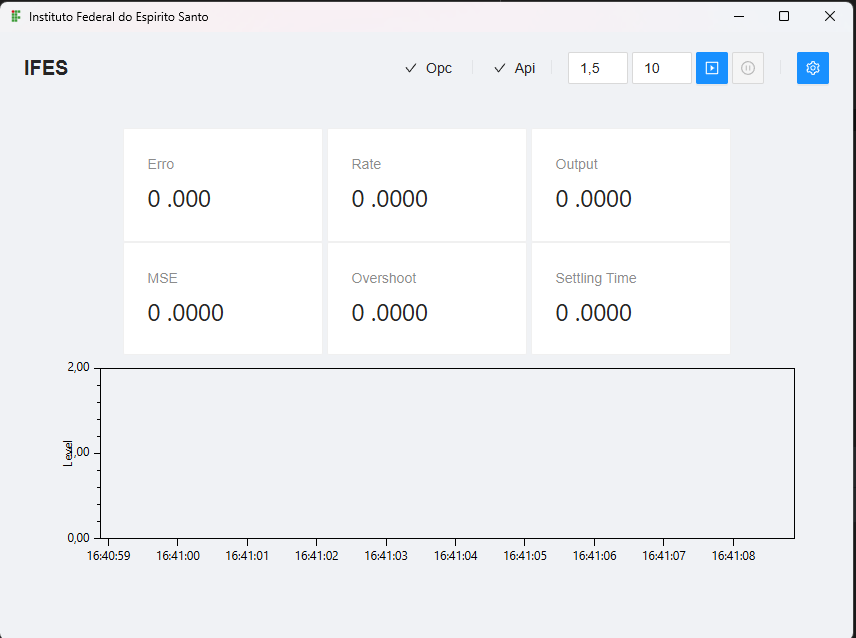
\includegraphics[width=1\textwidth]{figuras/imagens/ihm.png}
    
    {Fonte: Dias, 2025.}
    \label{fig:ihm}
\end{figure}

A IHM desenvolvida incorpora funcionalidades abrangentes de configuração e operação, proporcionando flexibilidade e facilidade de uso para diferentes cenários de aplicação. O sistema de configuração OPC permite ao usuário definir dinamicamente a URL do servidor OPC UA e especificar as tags de comunicação correspondentes às variáveis de processo. Esta funcionalidade elimina a necessidade de recompilação da aplicação para diferentes configurações de planta, facilitando a adaptação a diversos ambientes industriais e proporcionando portabilidade do sistema.

\begin{figure}[H]
    \centering
    \caption[Configuração do cliente OPC UA na interface da IHM.]{Configuração do cliente OPC UA na interface da IHM.}
    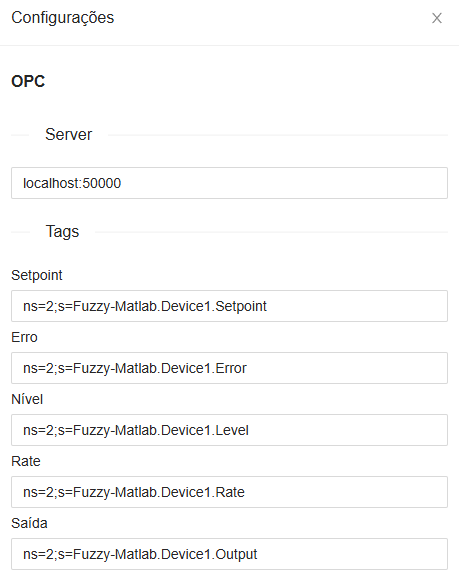
\includegraphics[width=0.7\textwidth]{figuras/imagens/ihm-config-opc.png}
    
    {Fonte: Dias, 2025.}
    \label{fig:ihmconfigopc}
\end{figure}

A interface oferece configuração do endpoint da API de controle Fuzzy, permitindo que o operador especifique o endereço do servidor onde a API está hospedada. Esta flexibilidade arquitetural possibilita distribuição geográfica dos componentes do sistema, onde a API pode operar em servidores dedicados ou em nuvem, enquanto a IHM mantém comunicação através de requisições HTTP padronizadas. A configuração dinâmica do endpoint facilita implementação em diferentes topologias de rede e estratégias de implantação.

\begin{figure}[H]
    \centering
    \caption[Configuração do endpoint da API de controle Fuzzy.]{Configuração do endpoint da API de controle Fuzzy.}
    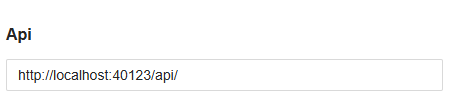
\includegraphics[width=0.7\textwidth]{figuras/imagens/ihm-config-api.png}
    
    {Fonte: Dias, 2025.}
    \label{fig:ihmconfigapi}
\end{figure}

O módulo de simulação integrado constitui funcionalidade essencial para validação e teste do sistema de controle. A IHM permite ao usuário definir o nível desejado (setpoint) e especificar o tempo de simulação em segundos, iniciando automaticamente o processo de controle com os parâmetros estabelecidos. Esta capacidade de simulação facilita análise de comportamento do sistema, otimização de parâmetros de controle e treinamento de operadores sem necessidade de intervenção direta na planta física.

\begin{figure}[H]
    \centering
    \caption[Interface de simulação integrada para testes do sistema de controle.]{Interface de simulação integrada para testes do sistema de controle.}
    
\includegraphics[]{figuras/imagens/ihm-simulation.png}
    
    {Fonte: Dias, 2025.}
    \label{fig:ihmsimulation}
\end{figure}

A visualização do status de conexão proporciona monitoramento contínuo da integridade das comunicações com o servidor OPC UA e a API de controle Fuzzy. Indicadores visuais em tempo real informam sobre o estado das conexões, facilitando identificação rápida de problemas de comunicação e implementação de estratégias de recuperação automática. Esta funcionalidade é fundamental para operação confiável em ambiente industrial, onde a continuidade da comunicação impacta diretamente a segurança e eficiência do processo.

\begin{figure}[H]
    \centering
    \caption[Monitoramento do status de conexão com servidor OPC UA e API.]{Monitoramento do status de conexão com servidor OPC UA e API.}
    
\includegraphics[]{figuras/imagens/ihm-service-status.png}
    
    {Fonte: Dias, 2025.}
    \label{fig:ihmsimulation}
\end{figure}

A interface gráfica integra todos estes elementos em layout intuitivo e funcional, proporcionando ao operador controle completo sobre o sistema distribuído através de uma única aplicação centralizada. A combinação destas funcionalidades resulta em ferramenta robusta para supervisão, controle e análise do sistema de controle de nível baseado em lógica Fuzzy integrado via protocolo OPC UA.